% Options for packages loaded elsewhere
\PassOptionsToPackage{unicode}{hyperref}
\PassOptionsToPackage{hyphens}{url}
\PassOptionsToPackage{dvipsnames,svgnames,x11names}{xcolor}
%
\documentclass[
  letterpaper,
  DIV=11,
  numbers=noendperiod]{scrartcl}

\usepackage{amsmath,amssymb}
\usepackage{lmodern}
\usepackage{iftex}
\ifPDFTeX
  \usepackage[T1]{fontenc}
  \usepackage[utf8]{inputenc}
  \usepackage{textcomp} % provide euro and other symbols
\else % if luatex or xetex
  \usepackage{unicode-math}
  \defaultfontfeatures{Scale=MatchLowercase}
  \defaultfontfeatures[\rmfamily]{Ligatures=TeX,Scale=1}
\fi
% Use upquote if available, for straight quotes in verbatim environments
\IfFileExists{upquote.sty}{\usepackage{upquote}}{}
\IfFileExists{microtype.sty}{% use microtype if available
  \usepackage[]{microtype}
  \UseMicrotypeSet[protrusion]{basicmath} % disable protrusion for tt fonts
}{}
\makeatletter
\@ifundefined{KOMAClassName}{% if non-KOMA class
  \IfFileExists{parskip.sty}{%
    \usepackage{parskip}
  }{% else
    \setlength{\parindent}{0pt}
    \setlength{\parskip}{6pt plus 2pt minus 1pt}}
}{% if KOMA class
  \KOMAoptions{parskip=half}}
\makeatother
\usepackage{xcolor}
\setlength{\emergencystretch}{3em} % prevent overfull lines
\setcounter{secnumdepth}{-\maxdimen} % remove section numbering
% Make \paragraph and \subparagraph free-standing
\ifx\paragraph\undefined\else
  \let\oldparagraph\paragraph
  \renewcommand{\paragraph}[1]{\oldparagraph{#1}\mbox{}}
\fi
\ifx\subparagraph\undefined\else
  \let\oldsubparagraph\subparagraph
  \renewcommand{\subparagraph}[1]{\oldsubparagraph{#1}\mbox{}}
\fi

\usepackage{color}
\usepackage{fancyvrb}
\newcommand{\VerbBar}{|}
\newcommand{\VERB}{\Verb[commandchars=\\\{\}]}
\DefineVerbatimEnvironment{Highlighting}{Verbatim}{commandchars=\\\{\}}
% Add ',fontsize=\small' for more characters per line
\usepackage{framed}
\definecolor{shadecolor}{RGB}{241,243,245}
\newenvironment{Shaded}{\begin{snugshade}}{\end{snugshade}}
\newcommand{\AlertTok}[1]{\textcolor[rgb]{0.68,0.00,0.00}{#1}}
\newcommand{\AnnotationTok}[1]{\textcolor[rgb]{0.37,0.37,0.37}{#1}}
\newcommand{\AttributeTok}[1]{\textcolor[rgb]{0.40,0.45,0.13}{#1}}
\newcommand{\BaseNTok}[1]{\textcolor[rgb]{0.68,0.00,0.00}{#1}}
\newcommand{\BuiltInTok}[1]{\textcolor[rgb]{0.00,0.23,0.31}{#1}}
\newcommand{\CharTok}[1]{\textcolor[rgb]{0.13,0.47,0.30}{#1}}
\newcommand{\CommentTok}[1]{\textcolor[rgb]{0.37,0.37,0.37}{#1}}
\newcommand{\CommentVarTok}[1]{\textcolor[rgb]{0.37,0.37,0.37}{\textit{#1}}}
\newcommand{\ConstantTok}[1]{\textcolor[rgb]{0.56,0.35,0.01}{#1}}
\newcommand{\ControlFlowTok}[1]{\textcolor[rgb]{0.00,0.23,0.31}{#1}}
\newcommand{\DataTypeTok}[1]{\textcolor[rgb]{0.68,0.00,0.00}{#1}}
\newcommand{\DecValTok}[1]{\textcolor[rgb]{0.68,0.00,0.00}{#1}}
\newcommand{\DocumentationTok}[1]{\textcolor[rgb]{0.37,0.37,0.37}{\textit{#1}}}
\newcommand{\ErrorTok}[1]{\textcolor[rgb]{0.68,0.00,0.00}{#1}}
\newcommand{\ExtensionTok}[1]{\textcolor[rgb]{0.00,0.23,0.31}{#1}}
\newcommand{\FloatTok}[1]{\textcolor[rgb]{0.68,0.00,0.00}{#1}}
\newcommand{\FunctionTok}[1]{\textcolor[rgb]{0.28,0.35,0.67}{#1}}
\newcommand{\ImportTok}[1]{\textcolor[rgb]{0.00,0.46,0.62}{#1}}
\newcommand{\InformationTok}[1]{\textcolor[rgb]{0.37,0.37,0.37}{#1}}
\newcommand{\KeywordTok}[1]{\textcolor[rgb]{0.00,0.23,0.31}{#1}}
\newcommand{\NormalTok}[1]{\textcolor[rgb]{0.00,0.23,0.31}{#1}}
\newcommand{\OperatorTok}[1]{\textcolor[rgb]{0.37,0.37,0.37}{#1}}
\newcommand{\OtherTok}[1]{\textcolor[rgb]{0.00,0.23,0.31}{#1}}
\newcommand{\PreprocessorTok}[1]{\textcolor[rgb]{0.68,0.00,0.00}{#1}}
\newcommand{\RegionMarkerTok}[1]{\textcolor[rgb]{0.00,0.23,0.31}{#1}}
\newcommand{\SpecialCharTok}[1]{\textcolor[rgb]{0.37,0.37,0.37}{#1}}
\newcommand{\SpecialStringTok}[1]{\textcolor[rgb]{0.13,0.47,0.30}{#1}}
\newcommand{\StringTok}[1]{\textcolor[rgb]{0.13,0.47,0.30}{#1}}
\newcommand{\VariableTok}[1]{\textcolor[rgb]{0.07,0.07,0.07}{#1}}
\newcommand{\VerbatimStringTok}[1]{\textcolor[rgb]{0.13,0.47,0.30}{#1}}
\newcommand{\WarningTok}[1]{\textcolor[rgb]{0.37,0.37,0.37}{\textit{#1}}}

\providecommand{\tightlist}{%
  \setlength{\itemsep}{0pt}\setlength{\parskip}{0pt}}\usepackage{longtable,booktabs,array}
\usepackage{calc} % for calculating minipage widths
% Correct order of tables after \paragraph or \subparagraph
\usepackage{etoolbox}
\makeatletter
\patchcmd\longtable{\par}{\if@noskipsec\mbox{}\fi\par}{}{}
\makeatother
% Allow footnotes in longtable head/foot
\IfFileExists{footnotehyper.sty}{\usepackage{footnotehyper}}{\usepackage{footnote}}
\makesavenoteenv{longtable}
\usepackage{graphicx}
\makeatletter
\def\maxwidth{\ifdim\Gin@nat@width>\linewidth\linewidth\else\Gin@nat@width\fi}
\def\maxheight{\ifdim\Gin@nat@height>\textheight\textheight\else\Gin@nat@height\fi}
\makeatother
% Scale images if necessary, so that they will not overflow the page
% margins by default, and it is still possible to overwrite the defaults
% using explicit options in \includegraphics[width, height, ...]{}
\setkeys{Gin}{width=\maxwidth,height=\maxheight,keepaspectratio}
% Set default figure placement to htbp
\makeatletter
\def\fps@figure{htbp}
\makeatother

\KOMAoption{captions}{tableheading}
\makeatletter
\makeatother
\makeatletter
\makeatother
\makeatletter
\@ifpackageloaded{caption}{}{\usepackage{caption}}
\AtBeginDocument{%
\ifdefined\contentsname
  \renewcommand*\contentsname{Table of contents}
\else
  \newcommand\contentsname{Table of contents}
\fi
\ifdefined\listfigurename
  \renewcommand*\listfigurename{List of Figures}
\else
  \newcommand\listfigurename{List of Figures}
\fi
\ifdefined\listtablename
  \renewcommand*\listtablename{List of Tables}
\else
  \newcommand\listtablename{List of Tables}
\fi
\ifdefined\figurename
  \renewcommand*\figurename{Figure}
\else
  \newcommand\figurename{Figure}
\fi
\ifdefined\tablename
  \renewcommand*\tablename{Table}
\else
  \newcommand\tablename{Table}
\fi
}
\@ifpackageloaded{float}{}{\usepackage{float}}
\floatstyle{ruled}
\@ifundefined{c@chapter}{\newfloat{codelisting}{h}{lop}}{\newfloat{codelisting}{h}{lop}[chapter]}
\floatname{codelisting}{Listing}
\newcommand*\listoflistings{\listof{codelisting}{List of Listings}}
\makeatother
\makeatletter
\@ifpackageloaded{caption}{}{\usepackage{caption}}
\@ifpackageloaded{subcaption}{}{\usepackage{subcaption}}
\makeatother
\makeatletter
\@ifpackageloaded{tcolorbox}{}{\usepackage[many]{tcolorbox}}
\makeatother
\makeatletter
\@ifundefined{shadecolor}{\definecolor{shadecolor}{rgb}{.97, .97, .97}}
\makeatother
\makeatletter
\makeatother
\ifLuaTeX
  \usepackage{selnolig}  % disable illegal ligatures
\fi
\IfFileExists{bookmark.sty}{\usepackage{bookmark}}{\usepackage{hyperref}}
\IfFileExists{xurl.sty}{\usepackage{xurl}}{} % add URL line breaks if available
\urlstyle{same} % disable monospaced font for URLs
\hypersetup{
  pdftitle={Lake Wobegon and the Panopticon},
  pdfauthor={Tom Slee},
  colorlinks=true,
  linkcolor={blue},
  filecolor={Maroon},
  citecolor={Blue},
  urlcolor={Blue},
  pdfcreator={LaTeX via pandoc}}

\title{Lake Wobegon and the Panopticon}
\author{Tom Slee}
\date{8/6/23}

\begin{document}
\maketitle
\begin{abstract}
An abstract
\end{abstract}
\ifdefined\Shaded\renewenvironment{Shaded}{\begin{tcolorbox}[boxrule=0pt, frame hidden, enhanced, borderline west={3pt}{0pt}{shadecolor}, breakable, sharp corners, interior hidden]}{\end{tcolorbox}}\fi

\hypertarget{lake-wobegon-and-the-panopticon-a-simulation-of-real-world-reputation-systems}{%
\section{Lake Wobegon and the Panopticon: a simulation of real-world
reputation
systems}\label{lake-wobegon-and-the-panopticon-a-simulation-of-real-world-reputation-systems}}

(Tom Slee, work in progress, 2015-11-08 and picked up again 2023-08-06.)

\hypertarget{introduction}{%
\subsection{Introduction}\label{introduction}}

Uber, Airbnb, and other ``sharing economy'' platforms build trust on
their platforms through \emph{reputations systems}, in which customers
rate service providers, and service providers rate customers. Rating
sites such as Yelp and TripAdvisor also rely on customer ratings to
recommend service providers such as hotels or restaurants.

Unlike Netflix, Amazon, and other product-focused recommender systems,
reputation systems involve people rating other people. A movie cannot
change in response to ratings, but people can and do respond to being
rated, and those doing the rating know that, and may take it into
account as they make their rating. At the technology level, reputation
systems may look like product recommender systems, but their social
meaning and behaviour is very different: far less linear, far more tied
to incentives that are not captured in the system itsef.

In the few years since they have become widespread, reputation systems
have shown two seemingly contradictory characteristics:

\begin{enumerate}
\def\labelenumi{\arabic{enumi}.}
\item
  (Lake Wobegon effect) Most ratings are very high. While ratings of
  Netflix movies peak around 3.5 out of 5, ratings on sharing economy
  websites are almost all positive (mostly five stars out of five). The
  oldest and most widely-studied reputation system is eBay, in which
  well over 90\% of ratings are positive; other systems such as
  BlaBlaCar show over 95\% of ratings as ``five out of five''.
\item
  (Panopticon effect). Service providers live in fear of a bad rating.
  They are very apprehensive that ratings given for the most frivolous
  of reasons by a customer they will never see again (and may not be
  able to identify) may wreck their earnings opportunities, either by
  outright removal from a platform or by pushing them down the rankings
  in search recommendations. Yelp restaurant owners rail at ``drive-by
  reviewers'' who damage their reputation; Uber drivers fear being
  ``deactivated'' (fired), which can happen if their rating slips below
  4.6 out of 5 (a rating that would be stellar for a movie).
\end{enumerate}

So are reputation systems effective or not? Here's the seeming
contradiction:

\begin{enumerate}
\def\labelenumi{\arabic{enumi}.}
\item
  The Lake Wobegon effect suggests that reputation systems are useless:
  they fail to discriminate between good and bad service providers (my
  take on this from a couple of years ago is
  \href{http://tomslee.net/2013/09/some-obvious-things-about-internet-reputation-systems.html}{here}).
  This suggestion is supported by quite a bit of recent empirical
  research which I have summarized in
  \href{http://www.orbooks.com/catalog/whats-yours-is-mine-by-tom-slee/}{MY
  NEW BOOK!}. Customers are treating reviews as a courtesy, rather than
  as an opportunity for objective assessment. Rather like a guest book,
  customers leave nice comments or say nothing at all.
\item
  The Panopticon effect suggests that rating systems are extremely
  effective in controlling the behaviour of service-providers, leading
  them to be customer-pleasing (sometimes extravagantly so) in order to
  avoid a damaging bad review.
\end{enumerate}

For some time, I've wondered whether these two effects can really both
exist at the same time, and if so what kind of incentives they introduce
for both customers and service providers. So I've built a simple model
reputation system that mimics both effects, and which shows that they
are not contradictory after all, but can co-exist. I use this model to
explore where the wider use of reputation systems is likely to take us.
The short version is this:

\begin{itemize}
\item
  If we separate the impersonal market transaction aspect of a
  customer-provider experience from the social aspect, then the Lake
  Wobegon effect and the Panopticon effect are not contradictory at all.
  The transactional aspect is shaped by the provider's \emph{competence}
  - a high competence leads to a good experience. The social aspect is
  shaped by the provider's (and customer's) \emph{attitude} - what kind
  of person they are.
\item
  Reputation systems do fail to discriminate among service providers of
  different competence, as the Lake Wobegon effect suggests.
\item
  Reputation systems encourage customers to behave in an entitled,
  demanding manner rather than engaging in respectful relationship with
  service providers.
\item
  Reputation systems encourage providers to adopt a servile attitude,
  indulging customers' whims and havnig to perform what sociologists
  call ``emotional labour''.
\item
  In summary, reputation systems do not improve quality so much as they
  impose a regime of servility on service providers.
\end{itemize}

\hypertarget{a-jupyter-notebook}{%
\subsection{A Jupyter notebook}\label{a-jupyter-notebook}}

This document is a \href{http://jupyter.org/}{Jupyter notebook}
(previously called an iPython notebook). The code for the model is
included as part of the document, and the graphs that show the results
are generated using the code in the document. If you want to reproduce
or extend this model, you can save the notebook, install the right
packages in a Python distribution, and run it on your own computer. In
addition to the requirements for Jupyter, you will need to install the
following packages in a Python 3 environment:

\begin{Shaded}
\begin{Highlighting}[]
\CommentTok{\# imports and setup}
\OperatorTok{\%}\NormalTok{matplotlib inline}
\ImportTok{import}\NormalTok{ random }\CommentTok{\# random number generation (included with pyuthon)}
\ImportTok{import}\NormalTok{ numpy }\ImportTok{as}\NormalTok{ np }\CommentTok{\# numerical libraries used by matplotlib}
\ImportTok{import}\NormalTok{ matplotlib }\CommentTok{\# plotting libraries}
\ImportTok{import}\NormalTok{ matplotlib.pyplot }\ImportTok{as}\NormalTok{ plt }\CommentTok{\# more plotting libraries}
\ImportTok{import}\NormalTok{ pandas }\ImportTok{as}\NormalTok{ pd }\CommentTok{\# data analysis library}
\end{Highlighting}
\end{Shaded}

\hypertarget{a-model-reputation-system}{%
\subsection{A model reputation system}\label{a-model-reputation-system}}

Rating people is different to rating movies. When we watch a movie the
relationship is one way (the movie does not interact with us), but when
we interact with others we enter into a two-way relationship. In some
cases this relationship is brief and not likely to be repeated: taking a
taxi or an Uber ride, eating in a fast-food restaurant in a city you are
passing through. In other cases the relationship is richer and repeated:
a stay at a Bed \& Breakfast or an Airbnb (in a case where the host is
present) may extend over days; a regular customer at a restaurant may
get to know the staff; a relationship with a hairdresser or car mechanic
may extend over years.

We now know, empirically, that the richer the customer-provider
relationship, the more likely the reputation system is to show a large
number of high ratings. When customers engage in a social relationship
rather than a simple market transaction, they are reluctant to give
negative ratings no matter what ther experience. The rating becomes, in
effect, one part of the customer-provider relationship rather than an
objective review.

Here, I try to build a model that captures the essence of customer and
provider behaviour in a simple reputation system. Customers have the
opportunity to rate providers after each exchange. Each exchange, in
turn, has components:

\begin{itemize}
\tightlist
\item
  a market exchange component, in which the customer's satisfaction
  depends on the provider's competence (provider competence is fixed).
\item
  a social component, in which the customer and provider engage in a
  give-and-take exchange that make extend over several interactions. To
  get technical for a moment, this social component is modelled as a
  repeated prisoner's dilemma, with the customer satisfaction and the
  provider satisfaction determined by the prisoner's dilemma payoffs.
  More details will become clear in the ``Code walkthrough'' sections
  below.
\end{itemize}

Most reputation systems use five-star ratings, but I simplify this to a
simple ``thumbs up/thumbs down'' binary option. Some reputation systems
allow providers to rate customers as well, and there are other variants
(are ratings private? do actors see the rating before they give their
own?) but even when service providers can rate customers there is an
asymmetry at work, in that the service provider has more at stake in the
rating. Adopting a one-way system is, I contend, a reasonable
simplification to produce a simple and generic model.

With that summary, the next section (\emph{Code walkthrough}) spells out
the details of the model, and the following section (\emph{Simulations})
runs several simulations of customers rating providers under various
conditions. The document then concludes.

\hypertarget{code-walkthrough}{%
\section{Code walkthrough}\label{code-walkthrough}}

Here is an annotated implementation of the model. If you don't know
python and are not interested in reading the code, the commentary should
spell out what's going on in this model reputation system. If you are
really not interested in this, the next section should be comprehensible
without reading this.

\hypertarget{parameters}{%
\subsection{Parameters}\label{parameters}}

Start with some constants that define the various things used elsewhere,
in an attempt to make the rest of the code more legible. You can
probably ignore these for now.

\begin{Shaded}
\begin{Highlighting}[]
\CommentTok{\# The choices available to the customer and provider in their social exchange}
\NormalTok{CHOICE\_GIVE }\OperatorTok{=} \DecValTok{0}
\NormalTok{CHOICE\_TAKE }\OperatorTok{=} \DecValTok{1}

\CommentTok{\# The payoffs in the prisoner\textquotesingle{}s dilemma. }
\NormalTok{PAYOFF\_GIVE\_VERSUS\_GIVE }\OperatorTok{=} \FloatTok{1.0} 
\NormalTok{PAYOFF\_GIVE\_VERSUS\_TAKE }\OperatorTok{=} \FloatTok{0.0}
\NormalTok{PAYOFF\_TAKE\_VERSUS\_GIVE }\OperatorTok{=} \FloatTok{1.5}
\NormalTok{PAYOFF\_TAKE\_VERSUS\_TAKE }\OperatorTok{=} \FloatTok{0.5}

\CommentTok{\# Attitudes (prisoner\textquotesingle{}s dilemma strategies)}
\NormalTok{ATTITUDE\_GIVE }\OperatorTok{=} \StringTok{"Give"}
\NormalTok{ATTITUDE\_GIVE\_AND\_TAKE }\OperatorTok{=} \StringTok{"Give \& Take"}
\NormalTok{ATTITUDE\_TAKE }\OperatorTok{=} \StringTok{"Take"}

\CommentTok{\# The customer rates the provider}
\NormalTok{RATING\_THUMBS\_UP }\OperatorTok{=} \FloatTok{1.0}
\NormalTok{RATING\_THUMBS\_DOWN }\OperatorTok{=} \OperatorTok{{-}}\FloatTok{1.0}
\end{Highlighting}
\end{Shaded}

\hypertarget{actors}{%
\subsection{Actors}\label{actors}}

Each customer or provider is an \emph{actor}. The Actor() object
represents the basic things we need to know about each customer and
provider.

Each actor has an \emph{attitude}, which is expressed in their choices.
(In game theoretic terms, each has a strategy expressed in the method
called choose()). An actor's attitude is fixed for the course of a
simulation. The attitude determines how the actor behaves during each
customer-provider interaction.

In each interaction, both actors choose one of GIVE or TAKE. Then they
actors gain or lose satisfaction depending on the choices, with the
``payoffs'' of satisfaction corresponding to the prisoner's dilemma
outcomes. If each actor chooses GIVE, that is better for each of them
than if both choose TAKE. However, the best of all for an actor is to
choose TAKE while the other actor chooses GIVE. To keep things simple,
only a very few attitudes are considered:

\begin{itemize}
\tightlist
\item
  Give: (provider only). The provider plays GIVE on every interaction.
  The provider is compliant, or servile (or ``customer is always
  right''), putting in full effort no matter how demanding the customer
  is. This is a provider prepared to endure the whims of the customer,
  engaging in ``emotional labour''.
\item
  Give \& Take: (customer or provider) This attitude seeks to encourage
  co-operative behaviour between customer and provider, and represents a
  collaborative, approach to self-governance (generous, but standing up
  for yourself if the other actor turns nasty). The customer plays GIVE
  on the first interaction, and after that plays by the ``golden rule'',
  returning GIVE with GIVE and TAKE with TAKE, (This is the ``Tit for
  Tat'' strategy for prisoner's dilemma).
\item
  Take: (customer only). This attitude simply plays TAKE at every
  opportunity, no matter how the provider behaves. This customer is
  looking out for themselves, no messing around.
\end{itemize}

The model can be extended easily so that both customers and providers
may adopt any of the three attitides (Give, Give \& Take, Take), and the
code does work for that, but I've not discussed it here.

So here are the Actor declarations:

\begin{Shaded}
\begin{Highlighting}[]
\KeywordTok{class}\NormalTok{ Actor():}
       
    \KeywordTok{def} \FunctionTok{\_\_init\_\_}\NormalTok{(}\VariableTok{self}\NormalTok{, actor\_attitude):}
        \VariableTok{self}\NormalTok{.attitude }\OperatorTok{=}\NormalTok{ actor\_attitude}
        \VariableTok{self}\NormalTok{.satisfaction }\OperatorTok{=} \FloatTok{0.0} \CommentTok{\# start off at zero satisfaction}
        \VariableTok{self}\NormalTok{.exchanges }\OperatorTok{=} \FloatTok{0.0} \CommentTok{\# how many exchanges has the actor seen}
        \VariableTok{self}\NormalTok{.previous\_choice }\OperatorTok{=} \VariableTok{None}
        \VariableTok{self}\NormalTok{.exchange\_score }\OperatorTok{=} \DecValTok{0} \CommentTok{\# score in a current exchange}
            
    \KeywordTok{def}\NormalTok{ choose(}\VariableTok{self}\NormalTok{, prev\_opponent\_choice):}
        \ControlFlowTok{if} \VariableTok{self}\NormalTok{.attitude }\OperatorTok{==}\NormalTok{ ATTITUDE\_GIVE:}
\NormalTok{            choice }\OperatorTok{=}\NormalTok{ CHOICE\_GIVE}
        \ControlFlowTok{elif} \VariableTok{self}\NormalTok{.attitude }\OperatorTok{==}\NormalTok{ ATTITUDE\_GIVE\_AND\_TAKE:}
            \ControlFlowTok{if}\NormalTok{ prev\_opponent\_choice }\KeywordTok{is} \VariableTok{None}\NormalTok{:}
\NormalTok{                choice }\OperatorTok{=}\NormalTok{ CHOICE\_GIVE }
            \ControlFlowTok{else}\NormalTok{:}
\NormalTok{                choice }\OperatorTok{=}\NormalTok{ prev\_opponent\_choice}
        \ControlFlowTok{elif} \VariableTok{self}\NormalTok{.attitude }\OperatorTok{==}\NormalTok{ ATTITUDE\_TAKE:}
\NormalTok{            choice }\OperatorTok{=}\NormalTok{ CHOICE\_TAKE}
        
        \CommentTok{\# Commented out, but you can re{-}instate if you want to explore this}
        \CommentTok{\# Notwithstanding the above, a fraction of choices are random, for both }
        \CommentTok{\# customer and provider. This represents misunderstanding and prevents}
        \CommentTok{\# artifical fragile equilibria from playing too big a part in the outcome}
        \CommentTok{\#if random.random() \textless{} noise\_fraction:}
        \CommentTok{\#    choice = random.choice([CHOICE\_GIVE, CHOICE\_TAKE])}

        \ControlFlowTok{return}\NormalTok{ choice}
\end{Highlighting}
\end{Shaded}

\hypertarget{customers-and-providers}{%
\subsection{Customers and providers}\label{customers-and-providers}}

Customers and providers are both Actors, but the provider has additional
characteristics: a \emph{competence} in providing their service, and a
\emph{reputation} (from the customers' assessments). The rating system
used here is a simple thumbs up or thumbs down choice, and it is also
helpful to track the number of each that a provider has accumulated: the
reputation can be computed from these as the fraction of thumbs up
ratings.

\begin{Shaded}
\begin{Highlighting}[]
\KeywordTok{class}\NormalTok{ Customer(Actor):}

    \KeywordTok{def} \FunctionTok{\_\_init\_\_}\NormalTok{(}\VariableTok{self}\NormalTok{, attitude):}
\NormalTok{        Actor.}\FunctionTok{\_\_init\_\_}\NormalTok{(}\VariableTok{self}\NormalTok{, attitude)}
        
\KeywordTok{class}\NormalTok{ Provider(Actor):}
    
    \KeywordTok{def} \FunctionTok{\_\_init\_\_}\NormalTok{(}\VariableTok{self}\NormalTok{, attitude):}
\NormalTok{        Actor.}\FunctionTok{\_\_init\_\_}\NormalTok{(}\VariableTok{self}\NormalTok{, attitude)}
        \VariableTok{self}\NormalTok{.rating }\OperatorTok{=} \FloatTok{0.0} \CommentTok{\# +1 for each THUMBS\_UP, {-}1 for each THUMBS\_DOWN}
        \VariableTok{self}\NormalTok{.rating\_count }\OperatorTok{=} \FloatTok{0.0}
        \VariableTok{self}\NormalTok{.competence }\OperatorTok{=} \VariableTok{None}
        
    \KeywordTok{def}\NormalTok{ reputation(}\VariableTok{self}\NormalTok{):}
        \CommentTok{\# Value in the range [{-}1, +1]}
        \ControlFlowTok{if} \VariableTok{self}\NormalTok{.rating\_count }\OperatorTok{\textgreater{}} \DecValTok{0}\NormalTok{:}
            \ControlFlowTok{return}\NormalTok{ (}\VariableTok{self}\NormalTok{.rating }\OperatorTok{/} \VariableTok{self}\NormalTok{.rating\_count)}
        \ControlFlowTok{else}\NormalTok{:}
            \ControlFlowTok{return} \DecValTok{0} \CommentTok{\# no ratings, no reputation}
\end{Highlighting}
\end{Shaded}

\hypertarget{a-customer-provider-interaction}{%
\subsection{A customer-provider
interaction}\label{a-customer-provider-interaction}}

Now we have customer and provider objects, we can model an interaction
between the two. Each individual interaction between a customer and a
provider is modelled as a single play of the prisoner's dilemma. The end
result of each interaction is a score for the customer and for the
provider representing their overall satisfaction with the interaction.

We'll see what kind of experience an interaction may represent after the
next definition, of an \emph{exchange}. Here is a function for an
individual interaction:

\begin{Shaded}
\begin{Highlighting}[]
\KeywordTok{def}\NormalTok{ interact(customer, provider):}
    \CommentTok{\# Each interaction in an exchange is a single play of the prisoner\textquotesingle{}s dilemma}
    \CommentTok{\# each actor makes a choice}
    \CommentTok{\# Prisoner\textquotesingle{}s dilemma choices: co{-}operate or defect}
\NormalTok{    customer\_choice }\OperatorTok{=}\NormalTok{ customer.choose(provider.previous\_choice)}
\NormalTok{    provider\_choice }\OperatorTok{=}\NormalTok{ provider.choose(customer.previous\_choice)}
    \CommentTok{\# now compute the payoffs}
    \ControlFlowTok{if}\NormalTok{ customer\_choice }\OperatorTok{==}\NormalTok{ CHOICE\_GIVE:}
        \ControlFlowTok{if}\NormalTok{ provider\_choice }\OperatorTok{==}\NormalTok{ CHOICE\_GIVE:}
\NormalTok{            customer\_score }\OperatorTok{=}\NormalTok{ PAYOFF\_GIVE\_VERSUS\_GIVE}
\NormalTok{            provider\_score }\OperatorTok{=}\NormalTok{ PAYOFF\_GIVE\_VERSUS\_GIVE}
        \ControlFlowTok{elif}\NormalTok{ provider\_choice }\OperatorTok{==}\NormalTok{ CHOICE\_TAKE:}
\NormalTok{            customer\_score }\OperatorTok{=}\NormalTok{ PAYOFF\_GIVE\_VERSUS\_TAKE}
\NormalTok{            provider\_score }\OperatorTok{=}\NormalTok{ PAYOFF\_TAKE\_VERSUS\_GIVE}
    \ControlFlowTok{elif}\NormalTok{ customer\_choice }\OperatorTok{==}\NormalTok{ CHOICE\_TAKE:}
        \ControlFlowTok{if}\NormalTok{ provider\_choice }\OperatorTok{==}\NormalTok{ CHOICE\_GIVE:}
\NormalTok{            customer\_score }\OperatorTok{=}\NormalTok{ PAYOFF\_TAKE\_VERSUS\_GIVE}
\NormalTok{            provider\_score }\OperatorTok{=}\NormalTok{ PAYOFF\_GIVE\_VERSUS\_TAKE}
        \ControlFlowTok{elif}\NormalTok{ provider\_choice }\OperatorTok{==}\NormalTok{ CHOICE\_TAKE:}
\NormalTok{            customer\_score }\OperatorTok{=}\NormalTok{ PAYOFF\_TAKE\_VERSUS\_TAKE}
\NormalTok{            provider\_score }\OperatorTok{=}\NormalTok{ PAYOFF\_TAKE\_VERSUS\_TAKE}
    \ControlFlowTok{return}\NormalTok{ (customer\_choice, provider\_choice, customer\_score, provider\_score)}
\end{Highlighting}
\end{Shaded}

\hypertarget{a-customer-provider-exchange}{%
\subsection{A customer-provider
exchange}\label{a-customer-provider-exchange}}

Each customer-provider exchange has a transactional component and a
social exchange component. The social exchange is made up of a number of
interactions (see above).

During each exchange the customer and provider gain or lose
\emph{satisfaction}. This satisfaction has a social component, which
marks their satisfaction (or otherwise) at the interaction itself, and a
transactional component, which is based on the provider's competence. If
the exchange is a guest staying with a host, then each interaction might
be the welcome, a meal, a conversation. If the exchange is a hairdresser
and a customer, then the exchange may represent a long relationship,
with each interaction being a visit. Of course, this is very schematic,
but the idea is that rich exchanges can be modelled with many
interactions, while a thin exchange may be a simple interaction.

At the end of the exchange, the customer has the opportunity to rate the
provider (THUMBS\_UP or THUMBS\_DOWN). How the customer rates depends on
the experience, and also on what kind of person the customer is (their
attitude).

A satisfying experience depends on the quality of service (represented
here as the competence of the provider), but also on the social aspect
of the interaction. Researchers have found that when dealing with
service providers, most customers care more about the service provider's
attitude than about their competence; more about what kind of person
they are than about the transaction.

Provider competence does matter when evaluating the provider, but the
importance of that aspect of the exchange is higher when the social
aspect is less important -- when there are few interactions in the
exchange -- and less important as the social aspect becomes richer.

If the customer decides they have had a good experience (based on the
outcome of both the social exchange and the market exchange), then the
customer will give a THUMBS\_UP rating. For customers who have had a bad
experience, the behaviour is different for each attitude:

\begin{itemize}
\tightlist
\item
  Customers playing Give \& Take, who treat the exchange as a
  relationship, do not give a bad rating if they have a bad experience;
  they simply give no rating at all, not wanting the awkwardness of
  engaging in critisicm. There is strong evidence that this is how many
  people actually behave in sharing economy reputation systems.
\item
  Customers playing Take, who focus on the market transaction will give
  a THUMBS\_DOWN rating if they have a bad experience.
\end{itemize}

Here is a function that describes a customer-provider exchange:

\begin{Shaded}
\begin{Highlighting}[]
\KeywordTok{def}\NormalTok{ experience\_exchange(customer, provider, interactions):}
    \CommentTok{\# an exchange between a customer and provider, consisting}
    \CommentTok{\# of multiple interactions}
    \ControlFlowTok{for}\NormalTok{ interaction }\KeywordTok{in} \BuiltInTok{range}\NormalTok{(interactions):}
\NormalTok{        (customer.previous\_choice, provider.previous\_choice,}
\NormalTok{         customer\_score, provider\_score) }\OperatorTok{=}\NormalTok{ interact(customer, }
\NormalTok{                                                    provider)}
\NormalTok{        customer.exchange\_score }\OperatorTok{+=}\NormalTok{ customer\_score}
\NormalTok{        provider.exchange\_score }\OperatorTok{+=}\NormalTok{ provider\_score}
    \CommentTok{\# normalize to a range between 0 and 1.5 (social bit is difficult)}
\NormalTok{    customer.exchange\_score }\OperatorTok{=}\NormalTok{ customer.exchange\_score }\OperatorTok{/}\NormalTok{ interactions}
\NormalTok{    provider.exchange\_score }\OperatorTok{=}\NormalTok{ provider.exchange\_score }\OperatorTok{/}\NormalTok{ interactions}
    
\KeywordTok{def}\NormalTok{ rate\_exchange(customer, provider, interactions):}
    \CommentTok{\# to conclude the exchange, the customer may rate the provider}
    \CommentTok{\# Competence becomes less importance as the number of interactions grows.}
    \CommentTok{\# Update utilities}
\NormalTok{    threshold\_score }\OperatorTok{=} \FloatTok{0.75}
\NormalTok{    mean\_competence }\OperatorTok{=} \FloatTok{0.5}
\NormalTok{    satisfaction\_threshold }\OperatorTok{=}\NormalTok{ (threshold\_score }\OperatorTok{+}\NormalTok{ mean\_competence)}\OperatorTok{/}\FloatTok{2.0}
    \CommentTok{\# track each actor\textquotesingle{}s overall satisfactin throughout all their exchanges}
\NormalTok{    tolerance }\OperatorTok{=} \FloatTok{0.00001} \CommentTok{\# deal with floating point comparisons}
    
    \ControlFlowTok{if}\NormalTok{ (customer.exchange\_score  }\OperatorTok{\textgreater{}}\NormalTok{ satisfaction\_threshold }\OperatorTok{{-}}\NormalTok{ tolerance):}
\NormalTok{        good\_experience }\OperatorTok{=} \VariableTok{True}
    \ControlFlowTok{else}\NormalTok{:}
\NormalTok{        good\_experience }\OperatorTok{=} \VariableTok{False}
    \ControlFlowTok{if}\NormalTok{ customer.attitude }\OperatorTok{==}\NormalTok{ ATTITUDE\_GIVE\_AND\_TAKE:}
        \CommentTok{\# only report good outcomes}
        \ControlFlowTok{if}\NormalTok{ good\_experience:}
\NormalTok{            provider.rating\_count }\OperatorTok{+=} \FloatTok{1.0}
\NormalTok{            provider.rating }\OperatorTok{+=}\NormalTok{ RATING\_THUMBS\_UP}
    \ControlFlowTok{elif}\NormalTok{ customer.attitude }\OperatorTok{==}\NormalTok{ ATTITUDE\_GIVE:}
        \CommentTok{\# always give a good rating, no matter what}
\NormalTok{        provider.rating\_count }\OperatorTok{+=} \FloatTok{1.0}
\NormalTok{        provider.rating }\OperatorTok{+=}\NormalTok{ RATING\_THUMBS\_UP}
    \ControlFlowTok{elif}\NormalTok{ customer.attitude }\OperatorTok{==}\NormalTok{ ATTITUDE\_TAKE:}
        \CommentTok{\# tell the truth}
\NormalTok{        provider.rating\_count }\OperatorTok{+=} \FloatTok{1.0}
        \ControlFlowTok{if}\NormalTok{ good\_experience:}
\NormalTok{            provider.rating }\OperatorTok{+=}\NormalTok{ RATING\_THUMBS\_UP}
        \ControlFlowTok{else}\NormalTok{:}
\NormalTok{            provider.rating }\OperatorTok{+=}\NormalTok{ RATING\_THUMBS\_DOWN}
            
\KeywordTok{def}\NormalTok{ exchange(customer, provider, interactions):}
    \ControlFlowTok{for}\NormalTok{ actor }\KeywordTok{in}\NormalTok{ [customer, provider]:}
\NormalTok{        actor.exchanges }\OperatorTok{+=} \FloatTok{1.0}
\NormalTok{        actor.exchange\_score }\OperatorTok{=} \FloatTok{0.0}
\NormalTok{        actor.previous\_choice }\OperatorTok{=} \VariableTok{None}
\NormalTok{    customer.exchange\_score }\OperatorTok{=}\NormalTok{ provider.competence }\CommentTok{\# transaction satisfaction}
    \ControlFlowTok{if}\NormalTok{ interactions }\OperatorTok{\textgreater{}} \DecValTok{0}\NormalTok{:}
\NormalTok{        experience\_exchange(customer, provider, interactions)}
\NormalTok{    rate\_exchange(customer, provider, interactions)}
\NormalTok{    customer.satisfaction }\OperatorTok{+=}\NormalTok{ customer.exchange\_score}
\NormalTok{    provider.satisfaction }\OperatorTok{+=}\NormalTok{ provider.exchange\_score}
\end{Highlighting}
\end{Shaded}

\hypertarget{a-rating-period}{%
\subsection{A rating period}\label{a-rating-period}}

Each simulation is run over a number of \emph{rating periods}. In each
rating period, every customer chooses a provider and they have an
exchange. Depending on the number of customers and providers, this may
mean that a provider undertakes several exchanges, one, or none.

The customer ratings are collected together as a \emph{reputation} score
for each provider, and the higher a provider's reputation, the better
their chance of being chosen by a customer in the next rating period. In
this way, the reputation feeds into the provider's life story.

Here is the function that describes a rating period:

\begin{Shaded}
\begin{Highlighting}[]
\KeywordTok{def}\NormalTok{ rating\_period(period, sim):}
    \CommentTok{\# Match up customers with providers: many customers may undertake an exchange with one provider}
    \CommentTok{\# in a single period.}
    \CommentTok{\# First assign ranges weighted by reputation}
\NormalTok{    maximum }\OperatorTok{=} \FloatTok{0.0}
\NormalTok{    store\_front\_max }\OperatorTok{=}\NormalTok{ [] }\CommentTok{\# a list of values partitioning a range so that exchanges can be matched}
    \ControlFlowTok{for}\NormalTok{ provider }\KeywordTok{in}\NormalTok{ sim.providers:}
\NormalTok{        maximum }\OperatorTok{+=}  \FloatTok{2.0} \OperatorTok{+}\NormalTok{ provider.reputation()}
\NormalTok{        store\_front\_max.append(maximum)}
        
    \CommentTok{\# Each customer chooses a provider and undertakes an exchange with them}
    \ControlFlowTok{for}\NormalTok{ customer }\KeywordTok{in}\NormalTok{ sim.customers:}
        \CommentTok{\# choose a value between zero and the maximum}
\NormalTok{        val }\OperatorTok{=}\NormalTok{ random.uniform(}\FloatTok{0.0}\NormalTok{, maximum)}
        \CommentTok{\# find which provider it is (inefficiently)}
        \ControlFlowTok{for}\NormalTok{ provider\_id }\KeywordTok{in} \BuiltInTok{range}\NormalTok{(}\BuiltInTok{len}\NormalTok{(sim.providers)):}
            \ControlFlowTok{if}\NormalTok{ val }\OperatorTok{\textless{}=}\NormalTok{ store\_front\_max[provider\_id]:}
                \ControlFlowTok{break}
\NormalTok{        exchange(customer, }
\NormalTok{                 sim.providers[provider\_id], }
\NormalTok{                 sim.interactions\_per\_exchange)}
\end{Highlighting}
\end{Shaded}

\hypertarget{a-complete-simulation-run}{%
\subsection{A complete simulation run}\label{a-complete-simulation-run}}

To run a complete simulation,the parameters that govern the simulation
are specified in the constructor for the Simulation oject, and then
Simulation.simulate() is called to carry out the simulation. The results
of the simulation are stored in the Simulation object so they can be
analyzed:

\begin{Shaded}
\begin{Highlighting}[]
\KeywordTok{class}\NormalTok{ Simulation():}

    \KeywordTok{def} \FunctionTok{\_\_init\_\_}\NormalTok{(}\VariableTok{self}\NormalTok{,}
\NormalTok{                customer\_counts,}
\NormalTok{                provider\_counts, }\CommentTok{\# dict of \{"attitude": count\}}
\NormalTok{                rating\_periods,}
\NormalTok{                interactions\_per\_exchange):}
        \VariableTok{self}\NormalTok{.rating\_periods }\OperatorTok{=}\NormalTok{ rating\_periods}
        \VariableTok{self}\NormalTok{.interactions\_per\_exchange }\OperatorTok{=}\NormalTok{ interactions\_per\_exchange}
        \VariableTok{self}\NormalTok{.customers }\OperatorTok{=}\NormalTok{ []}
        \VariableTok{self}\NormalTok{.customer\_attitudes }\OperatorTok{=}\NormalTok{ []}
\NormalTok{        random.seed(}\DecValTok{1}\NormalTok{)  }

        \ControlFlowTok{for}\NormalTok{ attitude, count }\KeywordTok{in}\NormalTok{ customer\_counts.items():}
            \ControlFlowTok{if}\NormalTok{ attitude }\KeywordTok{not} \KeywordTok{in} \VariableTok{self}\NormalTok{.customer\_attitudes:}
                \VariableTok{self}\NormalTok{.customer\_attitudes.append(attitude)}
            \ControlFlowTok{for}\NormalTok{ i }\KeywordTok{in} \BuiltInTok{range}\NormalTok{(count):}
                \VariableTok{self}\NormalTok{.customers.append(Customer(attitude))}
        \VariableTok{self}\NormalTok{.providers }\OperatorTok{=}\NormalTok{ []}
        \VariableTok{self}\NormalTok{.provider\_attitudes }\OperatorTok{=}\NormalTok{ []}
        
        \ControlFlowTok{for}\NormalTok{ attitude, count }\KeywordTok{in}\NormalTok{ provider\_counts.items():}
            \ControlFlowTok{if}\NormalTok{ attitude }\KeywordTok{not} \KeywordTok{in} \VariableTok{self}\NormalTok{.provider\_attitudes:}
                \VariableTok{self}\NormalTok{.provider\_attitudes.append(attitude)}
            \ControlFlowTok{for}\NormalTok{ i }\KeywordTok{in} \BuiltInTok{range}\NormalTok{(count):}
                \VariableTok{self}\NormalTok{.providers.append(Provider(attitude))}
        \CommentTok{\# assign competence uniformly in (0,1) but randomly }
\NormalTok{        shuffled\_providers }\OperatorTok{=} \BuiltInTok{list}\NormalTok{(}\BuiltInTok{range}\NormalTok{(}\BuiltInTok{len}\NormalTok{(}\VariableTok{self}\NormalTok{.providers)))}
\NormalTok{        random.shuffle(shuffled\_providers)}
        \ControlFlowTok{for}\NormalTok{ index, provider\_id }\KeywordTok{in} \BuiltInTok{enumerate}\NormalTok{(shuffled\_providers):}
            \VariableTok{self}\NormalTok{.providers[provider\_id].competence }\OperatorTok{=}\NormalTok{ ((index }\OperatorTok{+} \FloatTok{1.0}\NormalTok{) }\OperatorTok{/}
\NormalTok{                                                      (}\BuiltInTok{len}\NormalTok{(}\VariableTok{self}\NormalTok{.providers) }\OperatorTok{+} \FloatTok{1.0}\NormalTok{))}
        
    \KeywordTok{def}\NormalTok{ simulate(}\VariableTok{self}\NormalTok{):}
        \ControlFlowTok{for}\NormalTok{ period }\KeywordTok{in} \BuiltInTok{range}\NormalTok{(}\VariableTok{self}\NormalTok{.rating\_periods):}
\NormalTok{            rating\_period(period, }\VariableTok{self}\NormalTok{)}
\end{Highlighting}
\end{Shaded}

\hypertarget{plotting-functions}{%
\subsection{Plotting functions}\label{plotting-functions}}

These plotting functions generate graphs to help make sense of the
simulations. You can ignore them.

\begin{Shaded}
\begin{Highlighting}[]
\KeywordTok{def}\NormalTok{ plot\_by\_competence(sim):}
\NormalTok{    dfp }\OperatorTok{=}\NormalTok{ pd.DataFrame(\{}
        \StringTok{"attitude"}\NormalTok{: pd.Series([provider.attitude }\ControlFlowTok{for}\NormalTok{ provider }\KeywordTok{in}\NormalTok{ sim.providers]),}
        \StringTok{"competence"}\NormalTok{: pd.Series([provider.competence }\ControlFlowTok{for}\NormalTok{ provider }\KeywordTok{in}\NormalTok{ sim.providers]),}
        \StringTok{"satisfaction"}\NormalTok{: pd.Series([provider.satisfaction }\OperatorTok{/}\NormalTok{ provider.exchanges }
                              \ControlFlowTok{for}\NormalTok{ provider }\KeywordTok{in}\NormalTok{ sim.providers]),}
        \StringTok{"exchanges"}\NormalTok{: pd.Series([provider.exchanges }\ControlFlowTok{for}\NormalTok{ provider }\KeywordTok{in}\NormalTok{ sim.providers]),}
        \StringTok{"reputation"}\NormalTok{: pd.Series([provider.reputation() }\ControlFlowTok{for}\NormalTok{ provider }\KeywordTok{in}\NormalTok{ sim.providers]),}
\NormalTok{    \})}
\NormalTok{    markers }\OperatorTok{=}\NormalTok{ (}\StringTok{\textquotesingle{}o\textquotesingle{}}\NormalTok{, }\StringTok{\textquotesingle{}o\textquotesingle{}}\NormalTok{, }\StringTok{\textquotesingle{}*\textquotesingle{}}\NormalTok{)}
\NormalTok{    colors }\OperatorTok{=}\NormalTok{ (}\StringTok{\textquotesingle{}red\textquotesingle{}}\NormalTok{, }\StringTok{\textquotesingle{}blue\textquotesingle{}}\NormalTok{, }\StringTok{\textquotesingle{}green\textquotesingle{}}\NormalTok{)}
\NormalTok{    (marker\_size, width, opacity) }\OperatorTok{=}\NormalTok{ (}\DecValTok{50}\NormalTok{, }\FloatTok{0.8}\NormalTok{, }\FloatTok{0.6}\NormalTok{)}
\NormalTok{    fig, axes }\OperatorTok{=}\NormalTok{ plt.subplots(}\DecValTok{1}\NormalTok{, }\DecValTok{4}\NormalTok{, figsize}\OperatorTok{=}\NormalTok{(}\DecValTok{12}\NormalTok{, }\DecValTok{3}\NormalTok{)) }\CommentTok{\# rows, cols}
\NormalTok{    plt.style.use(}\StringTok{\textquotesingle{}ggplot\textquotesingle{}}\NormalTok{)}
    \CommentTok{\# plot one set of points on each axis, for each provider attitude}
    
\NormalTok{    dfp[}\StringTok{"reputation"}\NormalTok{].plot(kind}\OperatorTok{=}\StringTok{"hist"}\NormalTok{, alpha}\OperatorTok{=}\NormalTok{opacity, ax}\OperatorTok{=}\NormalTok{axes[}\DecValTok{0}\NormalTok{], xlim}\OperatorTok{=}\NormalTok{[}\OperatorTok{{-}}\FloatTok{1.1}\NormalTok{,}\FloatTok{1.1}\NormalTok{], title}\OperatorTok{=}\StringTok{"A1"}\NormalTok{)}
\NormalTok{    axes[}\DecValTok{0}\NormalTok{].set\_xlabel(}\StringTok{\textquotesingle{}Provider Reputation\textquotesingle{}}\NormalTok{)}
\NormalTok{    axes[}\DecValTok{0}\NormalTok{].set\_ylabel(}\StringTok{"Number of providers"}\NormalTok{)}
    \ControlFlowTok{for}\NormalTok{ index, attitude }\KeywordTok{in} \BuiltInTok{enumerate}\NormalTok{(sim.provider\_attitudes):}
\NormalTok{        dfp[dfp[}\StringTok{"attitude"}\NormalTok{] }\OperatorTok{==}\NormalTok{ attitude].plot(}
\NormalTok{            kind}\OperatorTok{=}\StringTok{"scatter"}\NormalTok{, x}\OperatorTok{=} \StringTok{"competence"}\NormalTok{, y }\OperatorTok{=} \StringTok{"satisfaction"}\NormalTok{, color}\OperatorTok{=}\NormalTok{colors[index], }
\NormalTok{            marker}\OperatorTok{=}\NormalTok{markers[index], s}\OperatorTok{=}\NormalTok{marker\_size, alpha}\OperatorTok{=}\NormalTok{opacity,}
\NormalTok{            ax}\OperatorTok{=}\NormalTok{axes[}\DecValTok{1}\NormalTok{], xlim}\OperatorTok{=}\NormalTok{[}\OperatorTok{{-}}\FloatTok{0.1}\NormalTok{,}\FloatTok{1.1}\NormalTok{], title}\OperatorTok{=}\StringTok{"A2"}\NormalTok{)}
\NormalTok{        dfp[dfp[}\StringTok{\textquotesingle{}attitude\textquotesingle{}}\NormalTok{] }\OperatorTok{==}\NormalTok{ attitude].plot(}
\NormalTok{            kind}\OperatorTok{=}\StringTok{"scatter"}\NormalTok{, x}\OperatorTok{=} \StringTok{"competence"}\NormalTok{, y }\OperatorTok{=} \StringTok{"reputation"}\NormalTok{, color}\OperatorTok{=}\NormalTok{colors[index], }
\NormalTok{            marker}\OperatorTok{=}\NormalTok{markers[index], s}\OperatorTok{=}\NormalTok{marker\_size, alpha}\OperatorTok{=}\NormalTok{opacity, }
\NormalTok{            ax}\OperatorTok{=}\NormalTok{axes[}\DecValTok{2}\NormalTok{], xlim}\OperatorTok{=}\NormalTok{[}\OperatorTok{{-}}\FloatTok{0.1}\NormalTok{,}\FloatTok{1.1}\NormalTok{], title}\OperatorTok{=}\StringTok{"A3"}\NormalTok{)}
\NormalTok{        dfp[dfp[}\StringTok{\textquotesingle{}attitude\textquotesingle{}}\NormalTok{] }\OperatorTok{==}\NormalTok{ attitude].plot(}
\NormalTok{            kind}\OperatorTok{=}\StringTok{"scatter"}\NormalTok{, x}\OperatorTok{=} \StringTok{"competence"}\NormalTok{, y }\OperatorTok{=} \StringTok{"exchanges"}\NormalTok{, color}\OperatorTok{=}\NormalTok{colors[index], }
\NormalTok{            marker}\OperatorTok{=}\NormalTok{markers[index], s}\OperatorTok{=}\NormalTok{marker\_size, alpha}\OperatorTok{=}\NormalTok{opacity, }
\NormalTok{            ax}\OperatorTok{=}\NormalTok{axes[}\DecValTok{3}\NormalTok{], label }\OperatorTok{=}\NormalTok{ attitude, xlim}\OperatorTok{=}\NormalTok{[}\OperatorTok{{-}}\FloatTok{0.1}\NormalTok{,}\FloatTok{1.1}\NormalTok{], title}\OperatorTok{=}\StringTok{"A4"}\NormalTok{)}
\NormalTok{    axes[}\DecValTok{1}\NormalTok{].set\_xlabel(}\StringTok{\textquotesingle{}Provider Competence\textquotesingle{}}\NormalTok{)}
\NormalTok{    axes[}\DecValTok{1}\NormalTok{].set\_ylabel(}\StringTok{\textquotesingle{}Provider Satisfaction\textquotesingle{}}\NormalTok{)}
\NormalTok{    axes[}\DecValTok{2}\NormalTok{].set\_xlabel(}\StringTok{\textquotesingle{}Provider Competence\textquotesingle{}}\NormalTok{)}
\NormalTok{    axes[}\DecValTok{2}\NormalTok{].set\_ylabel(}\StringTok{\textquotesingle{}Provider Reputation\textquotesingle{}}\NormalTok{)}
\NormalTok{    axes[}\DecValTok{3}\NormalTok{].set\_xlabel(}\StringTok{\textquotesingle{}Provider Competence\textquotesingle{}}\NormalTok{)}
\NormalTok{    axes[}\DecValTok{3}\NormalTok{].set\_ylabel(}\StringTok{\textquotesingle{}Exchanges\textquotesingle{}}\NormalTok{)}
\NormalTok{    axes[}\DecValTok{3}\NormalTok{].legend(fancybox}\OperatorTok{=}\VariableTok{True}\NormalTok{, shadow}\OperatorTok{=}\VariableTok{True}\NormalTok{, frameon}\OperatorTok{=}\VariableTok{True}\NormalTok{, }
\NormalTok{                   loc}\OperatorTok{=}\StringTok{\textquotesingle{}upper left\textquotesingle{}}\NormalTok{, bbox\_to\_anchor}\OperatorTok{=}\NormalTok{(}\FloatTok{1.05}\NormalTok{, }\FloatTok{1.0}\NormalTok{))}\OperatorTok{;}
\NormalTok{    plt.tight\_layout(pad}\OperatorTok{=}\FloatTok{0.4}\NormalTok{, w\_pad}\OperatorTok{=}\FloatTok{0.5}\NormalTok{, h\_pad}\OperatorTok{=}\FloatTok{1.0}\NormalTok{)}
\NormalTok{    plt.show()   }
    
\KeywordTok{def}\NormalTok{ plot\_by\_attitude(sim):}
\NormalTok{    dfc }\OperatorTok{=}\NormalTok{ pd.DataFrame(\{}
        \StringTok{"attitude"}\NormalTok{: pd.Series([customer.attitude }\ControlFlowTok{for}\NormalTok{ customer }\KeywordTok{in}\NormalTok{ sim.customers]),}
        \StringTok{"satisfaction"}\NormalTok{: pd.Series([customer.satisfaction }\OperatorTok{/}\NormalTok{ customer.exchanges }
                              \ControlFlowTok{for}\NormalTok{ customer }\KeywordTok{in}\NormalTok{ sim.customers]),}
        \StringTok{"exchanges"}\NormalTok{: pd.Series([customer.exchanges }\ControlFlowTok{for}\NormalTok{ customer }\KeywordTok{in}\NormalTok{ sim.customers]),}
\NormalTok{    \})}
\NormalTok{    dfp }\OperatorTok{=}\NormalTok{ pd.DataFrame(\{}
        \StringTok{"attitude"}\NormalTok{: pd.Series([provider.attitude }\ControlFlowTok{for}\NormalTok{ provider }\KeywordTok{in}\NormalTok{ sim.providers]),}
        \StringTok{"satisfaction"}\NormalTok{: pd.Series([provider.satisfaction }\OperatorTok{/}\NormalTok{ provider.exchanges }
                              \ControlFlowTok{for}\NormalTok{ provider }\KeywordTok{in}\NormalTok{ sim.providers]),}
        \StringTok{"reputation"}\NormalTok{: pd.Series([provider.reputation() }\ControlFlowTok{for}\NormalTok{ provider }\KeywordTok{in}\NormalTok{ sim.providers]),}
        \StringTok{"exchanges"}\NormalTok{: pd.Series([provider.exchanges }\ControlFlowTok{for}\NormalTok{ provider }\KeywordTok{in}\NormalTok{ sim.providers]),}
\NormalTok{    \})}
    \CommentTok{\# sns.set\_context("notebook", font\_scale=1.0, rc=\{"lines.linewidth": 2.5\})}
\NormalTok{    (width, opacity) }\OperatorTok{=}\NormalTok{ (}\FloatTok{0.4}\NormalTok{, }\FloatTok{0.6}\NormalTok{)}
\NormalTok{    fig, axes }\OperatorTok{=}\NormalTok{ plt.subplots(}\DecValTok{1}\NormalTok{, }\DecValTok{4}\NormalTok{, figsize}\OperatorTok{=}\NormalTok{(}\DecValTok{12}\NormalTok{, }\DecValTok{4}\NormalTok{)) }\CommentTok{\# rows, cols}
\NormalTok{    plt.setp(fig.axes, xticklabels}\OperatorTok{=}\NormalTok{sim.customer\_attitudes)}
\NormalTok{    plt.style.use(}\StringTok{\textquotesingle{}ggplot\textquotesingle{}}\NormalTok{)}
    \ControlFlowTok{for}\NormalTok{ i }\KeywordTok{in} \BuiltInTok{range}\NormalTok{(}\BuiltInTok{len}\NormalTok{(axes)):}
\NormalTok{        axes[i].set\_xlabel(}\StringTok{"Attitude"}\NormalTok{)}
\NormalTok{    df0 }\OperatorTok{=}\NormalTok{ pd.pivot\_table(dfc, index}\OperatorTok{=}\NormalTok{[}\StringTok{"attitude"}\NormalTok{], values}\OperatorTok{=}\StringTok{"satisfaction"}\NormalTok{)}
\NormalTok{    df0.plot(ax}\OperatorTok{=}\NormalTok{axes[}\DecValTok{0}\NormalTok{], kind}\OperatorTok{=}\StringTok{"bar"}\NormalTok{, alpha}\OperatorTok{=}\NormalTok{opacity, width}\OperatorTok{=}\NormalTok{width, title}\OperatorTok{=}\StringTok{"B1"}\NormalTok{)}
\NormalTok{    axes[}\DecValTok{0}\NormalTok{].set\_ylabel(}\StringTok{"Customer Satisfaction"}\NormalTok{)}
\NormalTok{    df1 }\OperatorTok{=}\NormalTok{ pd.pivot\_table(dfp, index}\OperatorTok{=}\NormalTok{[}\StringTok{"attitude"}\NormalTok{], values}\OperatorTok{=}\StringTok{"satisfaction"}\NormalTok{)}
\NormalTok{    df1.plot(ax}\OperatorTok{=}\NormalTok{axes[}\DecValTok{1}\NormalTok{], kind}\OperatorTok{=}\StringTok{"bar"}\NormalTok{, alpha}\OperatorTok{=}\NormalTok{opacity, width}\OperatorTok{=}\NormalTok{width, title}\OperatorTok{=}\StringTok{"B2"}\NormalTok{)}
\NormalTok{    axes[}\DecValTok{1}\NormalTok{].set\_ylabel(}\StringTok{"Provider Satisfaction"}\NormalTok{)}
\NormalTok{    df2 }\OperatorTok{=}\NormalTok{ pd.pivot\_table(dfp, index}\OperatorTok{=}\NormalTok{[}\StringTok{"attitude"}\NormalTok{], values}\OperatorTok{=}\StringTok{"reputation"}\NormalTok{)}
\NormalTok{    df2.plot(ax}\OperatorTok{=}\NormalTok{axes[}\DecValTok{2}\NormalTok{], kind}\OperatorTok{=}\StringTok{"bar"}\NormalTok{, alpha}\OperatorTok{=}\NormalTok{opacity, width}\OperatorTok{=}\NormalTok{width, ylim}\OperatorTok{=}\NormalTok{[}\OperatorTok{{-}}\FloatTok{1.0}\NormalTok{,}\FloatTok{1.0}\NormalTok{], title}\OperatorTok{=}\StringTok{"B3"}\NormalTok{)}
\NormalTok{    axes[}\DecValTok{2}\NormalTok{].set\_ylabel(}\StringTok{"Provider Reputation"}\NormalTok{)}
\NormalTok{    df3 }\OperatorTok{=}\NormalTok{ pd.pivot\_table(dfp, index}\OperatorTok{=}\NormalTok{[}\StringTok{"attitude"}\NormalTok{], values}\OperatorTok{=}\StringTok{"exchanges"}\NormalTok{)}
\NormalTok{    df3.plot(ax}\OperatorTok{=}\NormalTok{axes[}\DecValTok{3}\NormalTok{], kind}\OperatorTok{=}\StringTok{"bar"}\NormalTok{, alpha}\OperatorTok{=}\NormalTok{opacity, width}\OperatorTok{=}\NormalTok{width, title}\OperatorTok{=}\StringTok{"B4"}\NormalTok{)}
\NormalTok{    axes[}\DecValTok{3}\NormalTok{].set\_ylabel(}\StringTok{"Exchanges per Provider"}\NormalTok{)}
\NormalTok{    plt.tight\_layout(pad}\OperatorTok{=}\FloatTok{0.4}\NormalTok{, w\_pad}\OperatorTok{=}\FloatTok{0.5}\NormalTok{, h\_pad}\OperatorTok{=}\FloatTok{1.0}\NormalTok{)}
\NormalTok{    plt.show()      }
\end{Highlighting}
\end{Shaded}

\hypertarget{simulations}{%
\section{Simulations}\label{simulations}}

The model description is now complete, and we can run some simulations.
Recall that the point of this exercise is to investigate reputation
systems that display two seemingly-contradictory phenomena seen in the
real world: the Lake Wobegon effect in which (almost) everybody is given
a high rating, and the Panopticon effect in which service providers live
in fear of a bad rating. In particular:

\begin{itemize}
\tightlist
\item
  what qualities does such a system encourage in providers? (level of
  competence, attitude)
\item
  which customers are getting what they want?
\end{itemize}

\hypertarget{simulation-1-commodity-exchange}{%
\subsection{Simulation 1: commodity
exchange}\label{simulation-1-commodity-exchange}}

In the first simulation there is no social aspect to the exchange
(\emph{interactions\_per\_exchange = 0}) so the reputation of each
provider depends on their competence. The exchange is just like a market
transaction for a commodity: there is no back and forth between customer
and provider. The following code block assigns 240 customers to the Take
attitude (they will rate positive experiences and negative experiences),
distributes 80 providers evenly between ``Give \& Take'' and the more
indulgent ``Give'' attitudes, and runs them through 100 rating periods.

(Please ignore the pink warning box: this is a bug in matplotlib that
will be fixed soon).

\begin{Shaded}
\begin{Highlighting}[]
\NormalTok{sim }\OperatorTok{=}\NormalTok{ Simulation(}
\NormalTok{    customer\_counts }\OperatorTok{=}\NormalTok{ \{ATTITUDE\_TAKE: }\DecValTok{240}\NormalTok{\},}
\NormalTok{    provider\_counts }\OperatorTok{=}\NormalTok{ \{ATTITUDE\_GIVE: }\DecValTok{40}\NormalTok{, ATTITUDE\_GIVE\_AND\_TAKE: }\DecValTok{40}\NormalTok{\},}
\NormalTok{    rating\_periods }\OperatorTok{=} \DecValTok{100}\NormalTok{,}
\NormalTok{    interactions\_per\_exchange }\OperatorTok{=} \DecValTok{0}
\NormalTok{    )}
\NormalTok{sim.simulate()}
\NormalTok{plot\_by\_competence(sim)}
\NormalTok{plot\_by\_attitude(sim)}
\end{Highlighting}
\end{Shaded}

\begin{figure}[H]

{\centering 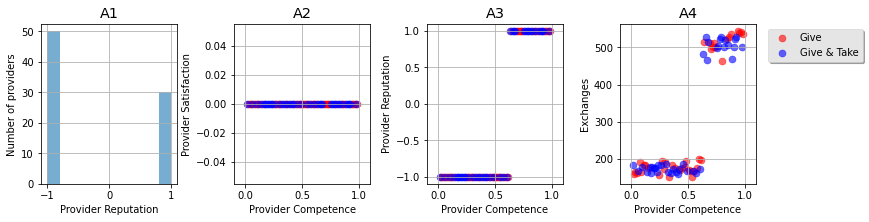
\includegraphics{provider-reputation_files/figure-pdf/cell-11-output-1.png}

}

\end{figure}

\begin{verbatim}
C:\Users\sleet\AppData\Local\Temp/ipykernel_16100/234662875.py:61: UserWarning: FixedFormatter should only be used together with FixedLocator
  plt.setp(fig.axes, xticklabels=sim.customer_attitudes)
\end{verbatim}

\begin{figure}[H]

{\centering 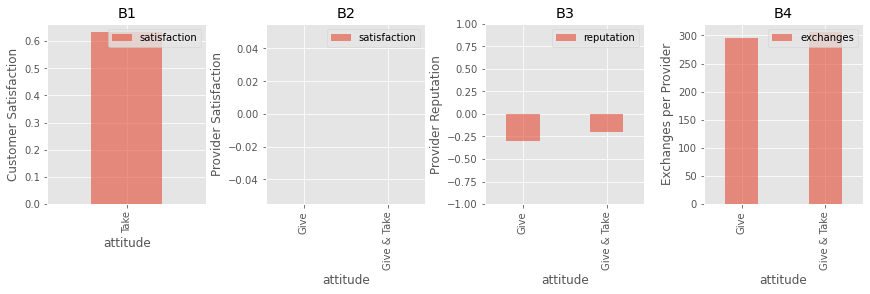
\includegraphics{provider-reputation_files/figure-pdf/cell-11-output-3.png}

}

\end{figure}

\hypertarget{simulation-1-commentary}{%
\subsubsection{Simulation 1 commentary}\label{simulation-1-commentary}}

In this case, attitude is irrelevant because there is no relationship.
A3 and B3 show that providers with a sub-par competence get rated badly
and have a reputation of minus-one, while providers with a
greater-than-average competence get rated with a thumbs-up by everyone.

This reputation carries over into the number of exchanges that each
provider gets: those with a good reputation get around 200 visits from
customers, while those with a good reputation mostly get about 500:
competent providers get more business (A4). Meanwhile, attitude is
irrelevant (B4).

In this special case the charts of provider satisfaction (A2, B2) are
irrelevant because provider satisfaction comes only from the social
aspect of the exchange, and in this case there is no social aspect.

This is how reputation systems are supposed to work, but it is not how
reputation systems work in the real world, where most providers get good
reputations and where the correlation of competence and reputation is
weak. Figure A1 shows a distribution of ratings in which many providers
have been given a bad reputation, completely unlike most real-world
reputation systems.

\hypertarget{simulation-2-lake-wobegon-ratings}{%
\subsection{Simulation 2: Lake Wobegon
ratings}\label{simulation-2-lake-wobegon-ratings}}

This simulation looks at the other extreme, where the provider's
competence is unimportant and the social relationship is all that
matters. Just as we don't rate friends based on their skills (except
perhaps in extreme circumstances), but on their personality and
integrity, so competence is not important here.

The simulation again has 240 customers and 80 providers (as weill all
the simulations) and the providers are again evenly distributed between
being ``Give \& Take'', and being servile (``Give''). Again there are
100 rating periods, but this time there are 25 interactions to every
exchange, so the social aspect of the exchange overwhelms the market
aspect.

\begin{Shaded}
\begin{Highlighting}[]
\NormalTok{sim }\OperatorTok{=}\NormalTok{ Simulation(}
\NormalTok{    customer\_counts }\OperatorTok{=}\NormalTok{ \{ATTITUDE\_GIVE\_AND\_TAKE: }\DecValTok{240}\NormalTok{\},}
\NormalTok{    provider\_counts }\OperatorTok{=}\NormalTok{ \{ATTITUDE\_GIVE\_AND\_TAKE: }\DecValTok{40}\NormalTok{, ATTITUDE\_GIVE: }\DecValTok{40}\NormalTok{\},}
\NormalTok{    rating\_periods }\OperatorTok{=} \DecValTok{100}\NormalTok{,}
\NormalTok{    interactions\_per\_exchange }\OperatorTok{=} \DecValTok{25}
\NormalTok{    )}
\NormalTok{sim.simulate()}
\NormalTok{plot\_by\_competence(sim)}
\NormalTok{plot\_by\_attitude(sim)}
\end{Highlighting}
\end{Shaded}

\begin{figure}[H]

{\centering 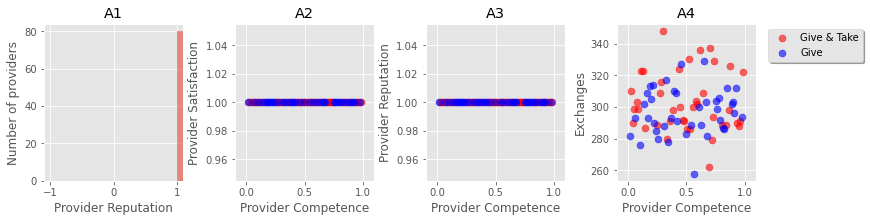
\includegraphics{provider-reputation_files/figure-pdf/cell-12-output-1.png}

}

\end{figure}

\begin{verbatim}
C:\Users\sleet\AppData\Local\Temp/ipykernel_16100/234662875.py:61: UserWarning: FixedFormatter should only be used together with FixedLocator
  plt.setp(fig.axes, xticklabels=sim.customer_attitudes)
\end{verbatim}

\begin{figure}[H]

{\centering 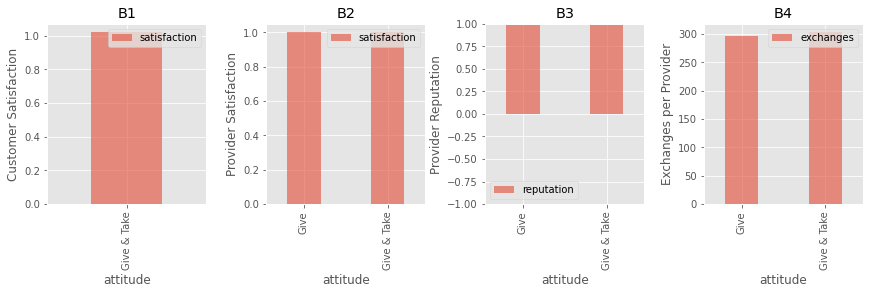
\includegraphics{provider-reputation_files/figure-pdf/cell-12-output-3.png}

}

\end{figure}

\hypertarget{simulation-2-commentary}{%
\subsubsection{Simulation 2 commentary}\label{simulation-2-commentary}}

A1 shows that all providers have a very high reputation (Lake Wobegon).
A3 confirms that this high reputation means nothing: it does not
distinguish based on competence or on attitude, because the ``Give \&
Take'' customers only give good ratings, keeping bad experiences to
themselves. The reputation system is weak, and A4 shows that there is no
correlation between competence, attitude, and the number of exchanges a
provider gets.

But that does not mean that things are bad. B1 shows that customers get
a high level of satisfaction (0.9) from the relationship aspect of the
exchange - the mutual cooperation of provider and customer. B2 shows
that providers also do well (0.7 or more). So things are good, but
different. This describes a self-governing system, where reputation does
not matter, but customer and provider each induce the other to be
generous.

\hypertarget{simulation-3-introducing-entitled-customers}{%
\subsection{Simulation 3: introducing entitled
customers}\label{simulation-3-introducing-entitled-customers}}

Now make one change: instead of all customers displaying a Give \& Take
attitude, one in ten will be demanding, and will play TAKE on all
aspects of the exchange. Even though the exchange is primarily social,
they may rate positively if they get a good outcome (which means, if the
provider is compliant) or badly if they do not.

\begin{Shaded}
\begin{Highlighting}[]
\NormalTok{sim }\OperatorTok{=}\NormalTok{ Simulation(}
\NormalTok{    customer\_counts }\OperatorTok{=}\NormalTok{ \{ATTITUDE\_GIVE\_AND\_TAKE: }\DecValTok{216}\NormalTok{, ATTITUDE\_TAKE: }\DecValTok{24}\NormalTok{\},}
\NormalTok{    provider\_counts }\OperatorTok{=}\NormalTok{ \{ATTITUDE\_GIVE\_AND\_TAKE: }\DecValTok{40}\NormalTok{, ATTITUDE\_GIVE: }\DecValTok{40}\NormalTok{\},}
\NormalTok{    rating\_periods }\OperatorTok{=} \DecValTok{100}\NormalTok{,}
\NormalTok{    interactions\_per\_exchange }\OperatorTok{=} \DecValTok{25}
\NormalTok{    )}
\NormalTok{sim.simulate()}
\NormalTok{plot\_by\_competence(sim)}
\NormalTok{plot\_by\_attitude(sim)}
\end{Highlighting}
\end{Shaded}

\begin{figure}[H]

{\centering 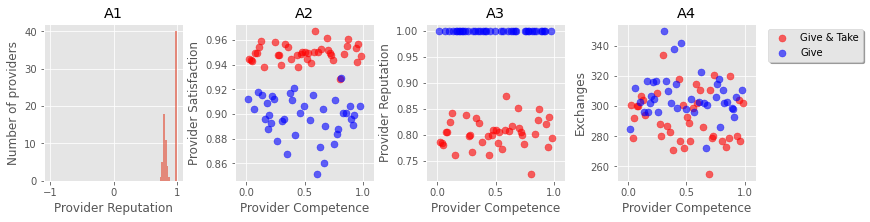
\includegraphics{provider-reputation_files/figure-pdf/cell-13-output-1.png}

}

\end{figure}

\begin{verbatim}
C:\Users\sleet\AppData\Local\Temp/ipykernel_16100/234662875.py:61: UserWarning: FixedFormatter should only be used together with FixedLocator
  plt.setp(fig.axes, xticklabels=sim.customer_attitudes)
\end{verbatim}

\begin{figure}[H]

{\centering 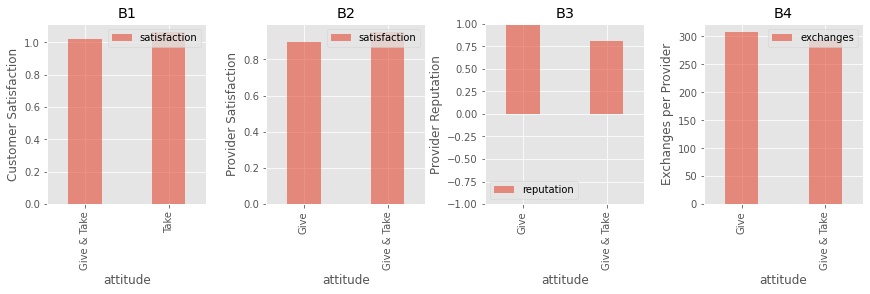
\includegraphics{provider-reputation_files/figure-pdf/cell-13-output-3.png}

}

\end{figure}

\hypertarget{simulation-3-commentary}{%
\subsubsection{Simulation 3 commentary}\label{simulation-3-commentary}}

A1 shows a distribution of reputations that is similar to many sharing
economy reputation systems: a large number of top-rated providers, and a
few who are rated slightly less than perfect. A3 shows that the
distinction has nothing to do with provider competence, but is shaped by
the provider's attitude, with a ``Give'' attitude leading to a higher
reputation than a ``Give \& Take'' attitude.

Those providers who look for a reciprocal relationship get thumbs up
from similar customers, but they get thumbs down from the entitled
customers: after the provider response to the customer's initial TAKE
with a TAKE of their own, the relationship goes sour and settles in to a
low-scoring ``Take - Take'' trap. Those providers who are indulgent
(``Give'') get exploited: they have to put up with the continual Take
choices of the customer with a smile, but do get rewarded with a higher
reputation (A3, B3), and so get a little more business (A4, B4).

A2 and B2 shows that the reciprocal providers have a slightly better
experience than compliant providers.

B1 shows that the two customer types have a similar level of
satisfaction. The reciprocal customers do well with all providers, while
the entitled customers do less well with the reciprocal providers (they
do not get along), but happily exploit the indulgence of the compliant
providers.

So what is happening here is just what we see in most service reputation
systems. From the point of view of the rating system provider itself,
this is a better result: the entitled customers are the ones behaving
just as they should - not being biased by their relationship with the
service provider, delivering an ``honest'' assessment of the quality of
their experience. The collaborative customers, building a relationship
with the provider, and reluctant to snitch on them through the rating
system, are the ones that are in the wrong from the reputation system
point of view.

Seen from anywhere other than the perspective of the platform provider,
this setup panders to demanding consumers by requiring service providers
to engage in emotional labour.

\hypertarget{simulation-4-more-honest-customers}{%
\subsection{Simulation 4: more ``honest''
customers}\label{simulation-4-more-honest-customers}}

This final simulation increases the proportion of entitled customers (or
``honest raters'' as the platform provider would see it) to see what
happens as the rating system ``improves''.

If Simulation 3 describes the way that reputation systems currently
work, Simulation 4 describes the way that the platform owners (sharing
economy companies and rating providers) would like them to work: they
expect customers to be ``honest'' - report good and bad experiences, and
to maintain an emotional distance from their service provider (to avoid
``bias''). These ideal customers are not committed to the social
exchange (not ``Give \& Take''), but instead treat the experience as one
to be judged.

\begin{Shaded}
\begin{Highlighting}[]
\NormalTok{sim }\OperatorTok{=}\NormalTok{ Simulation(}
\NormalTok{    customer\_counts }\OperatorTok{=}\NormalTok{ \{ATTITUDE\_GIVE\_AND\_TAKE: }\DecValTok{120}\NormalTok{, ATTITUDE\_TAKE: }\DecValTok{120}\NormalTok{\},}
\NormalTok{    provider\_counts }\OperatorTok{=}\NormalTok{ \{ATTITUDE\_GIVE\_AND\_TAKE: }\DecValTok{40}\NormalTok{, ATTITUDE\_GIVE: }\DecValTok{40}\NormalTok{\},}
\NormalTok{    rating\_periods }\OperatorTok{=} \DecValTok{100}\NormalTok{,}
\NormalTok{    interactions\_per\_exchange }\OperatorTok{=} \DecValTok{25}
\NormalTok{    )}
\NormalTok{sim.simulate()}
\NormalTok{plot\_by\_competence(sim)}
\NormalTok{plot\_by\_attitude(sim)}
\end{Highlighting}
\end{Shaded}

\begin{figure}[H]

{\centering 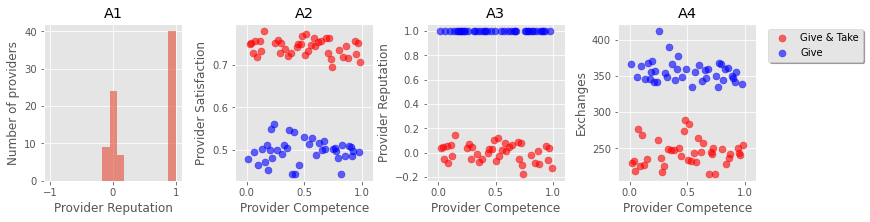
\includegraphics{provider-reputation_files/figure-pdf/cell-14-output-1.png}

}

\end{figure}

\begin{verbatim}
C:\Users\sleet\AppData\Local\Temp/ipykernel_16100/234662875.py:61: UserWarning: FixedFormatter should only be used together with FixedLocator
  plt.setp(fig.axes, xticklabels=sim.customer_attitudes)
\end{verbatim}

\begin{figure}[H]

{\centering 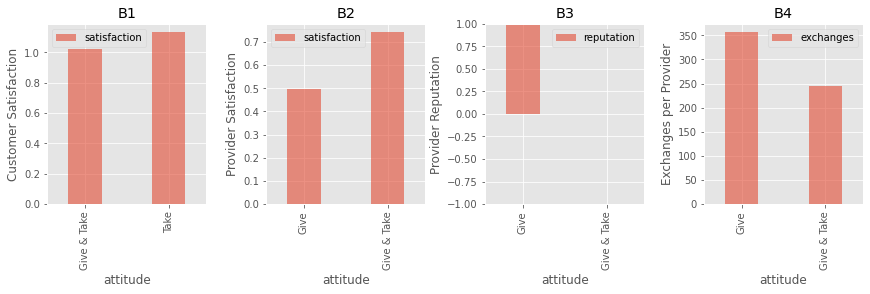
\includegraphics{provider-reputation_files/figure-pdf/cell-14-output-3.png}

}

\end{figure}

\hypertarget{simulation-4-commentary}{%
\subsubsection{Simulation 4 commentary}\label{simulation-4-commentary}}

The split between Give \& Take providers and compliant providers has
grown. A2 and B2 show that compliant providers are having a miserable
experience (their satisfaction is lower than that of the Give \& Take
providers), but their reputation is a lot better (thanks to the entitled
customers) and so their business prospers do better (more exchanges).
The compliant providers are ruling the roost. B1 shows that entitled
customers are having more satisfying experiences. The high reputation
for compliant providers is rewarded with higher traffic, and entitled
customers do very well from compliant providers by exploiting their
indulgent behaviour.

\hypertarget{conclusion}{%
\section{Conclusion}\label{conclusion}}

The fact that Simulation 2 gives a rating distribution far more like
current sharing economy reputation systems than Simulation 1
demonstrates the important role of social exchange compared to a pure
market or transactional exchange in most customer--service provider
exchanges. It is this social exchange that is at the root of the Lake
Wobegon effect, where all providers are above average. Reputation
systems do indeed fail to discriminate on the basis of competence
(quality).

Simulation 3 shows that a small number of entitled customers can induce
a Panopticon effect. Service providers who engage in Give \& Take
exchanges with their customers (even very competent ones) risk being
given a negative review, which will damage their business. The
incentives of the reputation system encourage providers to indulge their
customers, in order to avoid this unlikely but damaging judgement.

Simulation 4 shows that, if reputation systems spread and customers
become used to rating people in an ``honest'' fashion, we are building a
terrible world for service providers. They must engage in emotional
labour, catering to customer whims, or risk their livelihood. The
Panopticon is here. The reputation systems continue to fail, it should
be noted, to discriminate based on the competence of the service
provider -- instead of changing quality, they change attitude.

The Lake Wobegon effect and the Panopticon effect can coexist, and are
coexisting. Reputation systems as they currently stand are failing to
discriminate based on quality. But there is only one thing worse than a
reputation system that doesn't work, and that's a reputation system that
works: Simulation 4 shows a dystopic future for service providers, in
which their careers are being shaped by reputation systems that are not
working as advertised, but are working to compel compliance.



\end{document}
